\chapter{IaaS and PaaS bootstrapping}\label{iaas-and-paas-bootstrapping}

In order to deploy a containerized application in staging or production, first there is the need of a suitable environment.  While a development environment only need of launching one application with limited usage (only the developer itself) exposing only at localhost, a production environment has much more prerequisites.  The application should be always available, supporting many concurrent users from a public DNS, and lastly many instances of the same application could run at the same time.

This chapter will cover the process of launching the platform (in the PaaS way) on top of an IaaS from a cloud provider, delegating to the next one the internals of this PaaS and how running applications on top of it.

Usually a non trivial production environment is not composed by a unique machine but it's distributed on more hosts collaborate each other to enable further possibilities.  In particular CoreOS, Kubernetes and OpenShift were born with native concept of cluster, in which it's possible classify the hosts in 2 roles:
\begin{itemize}
\item \textit{master} (M), a control host of the life of the whole cluster;
\item \textit{node} (N), a worker host on which run applications.
\end{itemize}

Then, looking at the possible clustered architectures provided, as shown in figure 4.1 has been divided 3 kind of possible cluster architectures depends of configuration complexity level:
\begin{itemize}
\item a single host with both master and node roles;
\item 1 master and multiple nodes;
\item multiple masters and nodes.
\end{itemize}

\begin{figure}[htbp]
\centering
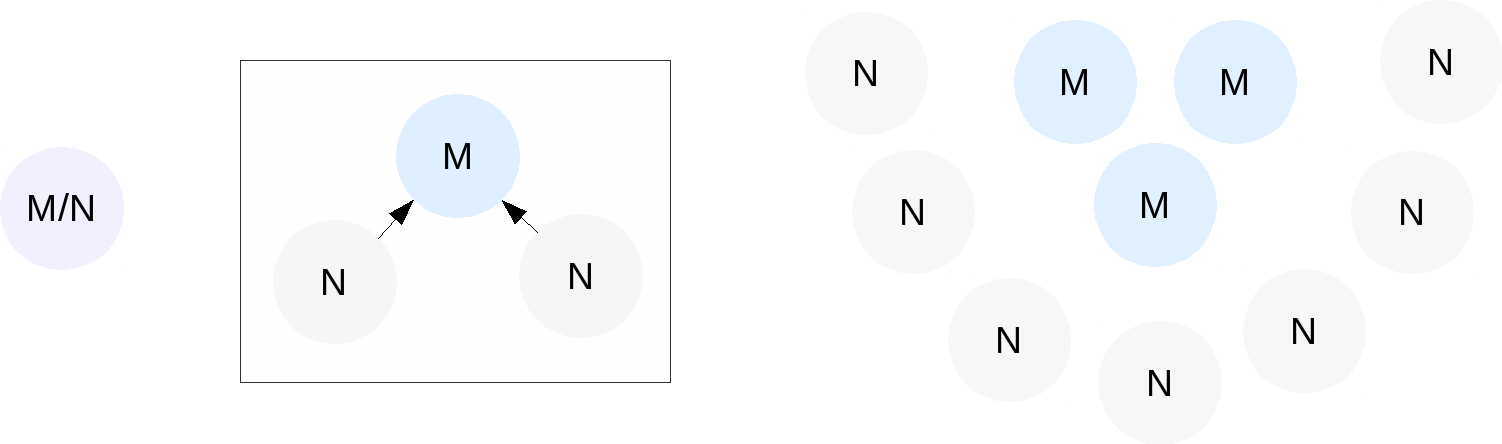
\includegraphics{media/ch4-clusters.png}
\caption{Cluster variants}
\end{figure}

While the first one represents only a very basic limit case, and the last one an advanced configuration for medium to big environments, the second one fits the needs of a small environment, with a balance between roles isolation, low cluster overhead and configuration complexity.  In particular will be used the simplest sub-case with a total of 3 hosts:  1 master and 2 nodes.

\section{IaaS Providers}\label{iaas-providers}

The first step is choice an IaaS provider for machines (compute and storage) and networking.  Even if there is no theoretical need of virtualization, there is a pragmatical one since the resources needed for every host is only a fraction of a whole modern physical server.  It's relevant note that instead of using virtualization for separating applications, in this case it will used for take only a part of the resource of a physical server, and containers represent the level for isolating the applications.  In conclusion, in order to pull up the cluster, there will take 3 VMs from a cloud provider.

In summary, the needed features of the cloud provider are:
\begin{itemize}
\item CoreOS native support, with additional possibility of customizing images;
\item integration with existing tools (\textit{Terraform} in particular);
\item simple plans avoiding proprietary or provider-specific services;
\item relatively economic.
\end{itemize}

Then will be useful some cluster-oriented features like:
\begin{itemize}
\item private network;
\item low-cost for intra-cluster traffic.
\end{itemize}

In additional extra features could be the integration of DNS Management in order to cover all the infrastructure-level services.

Digital Ocean\footnote{https://www.digitalocean.com/} (DO), built on top of free software \textit{QEMU} and \textit{KVM}, matches all the above points.

The master host doesn't run applications, and its sizing depends on number of nodes and containers to manage, while the sizing of nodes depends on  resources needed for applications.  After looking at Digital Ocean offer\footnote{https://www.digitalocean.com/pricing/}, the following plans were chosen:

\begin{itemize}
\item 1 master with 1 core, 1GB memory and 30GB SSD;
\item 2 nodes with 2 cores, 2GB memory and 40GB SSD each one.
\end{itemize}

For a total of 5 cores, 5GB memory and 110GB SSD.  Finally, the cluster has to be composed by hosts in the same data center in order to keeping the latency in intra-cluster communication as low as possible.

\section{Provisioning of IaaS}\label{provisioning-of-iaas}

Using a PaaS means a lot of automation and good practices applied in deploying applications.  For keeping a similar level of automation in provisioning all the lower stack than applications, there is need of additional tools.

In particular the tasks should be:
\begin{itemize}
\item describe the resource of infrastructure, possibly in a declarative way;
\item resolve the dependencies graph of infrastructure resources;
\item communicate with the provider through APIs (and auth token) doing the necessary operations;
\item connecting via SSH to the hosts for bootstrapping;
\item setting up the public DNS in order to point to a specific node of the cluster.
\end{itemize}

\textit{Ansible} and \textit{SaltStack} are popular choices today since includes several modules for lower-level operations (cloud provisioning) but also higher-level ones (application deployment and configuration management).  Since the applications are managed entirely by the PaaS as will be shown in next chapter, these tools are over sized.

\textit{Terraform} is a more minimal CLI-based tool, focuses only on cloud infrastructure provisioning on which results more productive and powerful.  Terraform applies the changes based on:
\begin{itemize}
\item actual state:  description of current resource states;
\item desired state:  description of resource states.
\end{itemize}

With these in mind, Terraform processes the data doing necessary operations aiming to keep from "actual state" to "desired state".  A basic example could be:
\begin{itemize}
\item actual state:  there is no machines;
\item desired state:  there is need of 3 machines.
\end{itemize}

So Terraform will communicate to provider via APIs in order to pull up 3 machines, then after the creation of these machines, their data (public IP, etc) will be stored as "actual state".  Then, if there is no need of a VMs, it's only necessary change the desired state and re-apply Terraform.

This approach of Terraform enables the possibility of so-called \textit{Infrastructure as Code} (IaC), that consists in versioning this files contains the states in order to tracks the infrastructure evolution, just as it is a common software project.  This represent a more structured, deterministic and reproducible way to infrastructure management.

In addition, Terraform could be used for enabling powerful features like horizontal host-level auto-scaling, varying the cardinality of the cluster in response to global load changes.

The resources (in execution order) are:
\begin{enumerate}
\item access token for Digital Ocean APIs (previously generated by provider Web UI);
\item upload temporary public SSH key (used for connection to hosts);
\item PaaS bootstrapping, regarding VMs and configuration (will be covered in the next sub-chapter);
\item DNS management for \textit{befaircloud.me}, a dedicated domain for this project, through Digital Ocean DNS service;
\item pointing \textit{*.befaircloud.me} A-type record to the first node.
\end{enumerate}

In addition, some variables for parametrization are used for a more DRY configuration.

Figure 4.2 shows an overview of automated infrastructure provisioning via Terraform.

\begin{figure}[htbp]
\centering
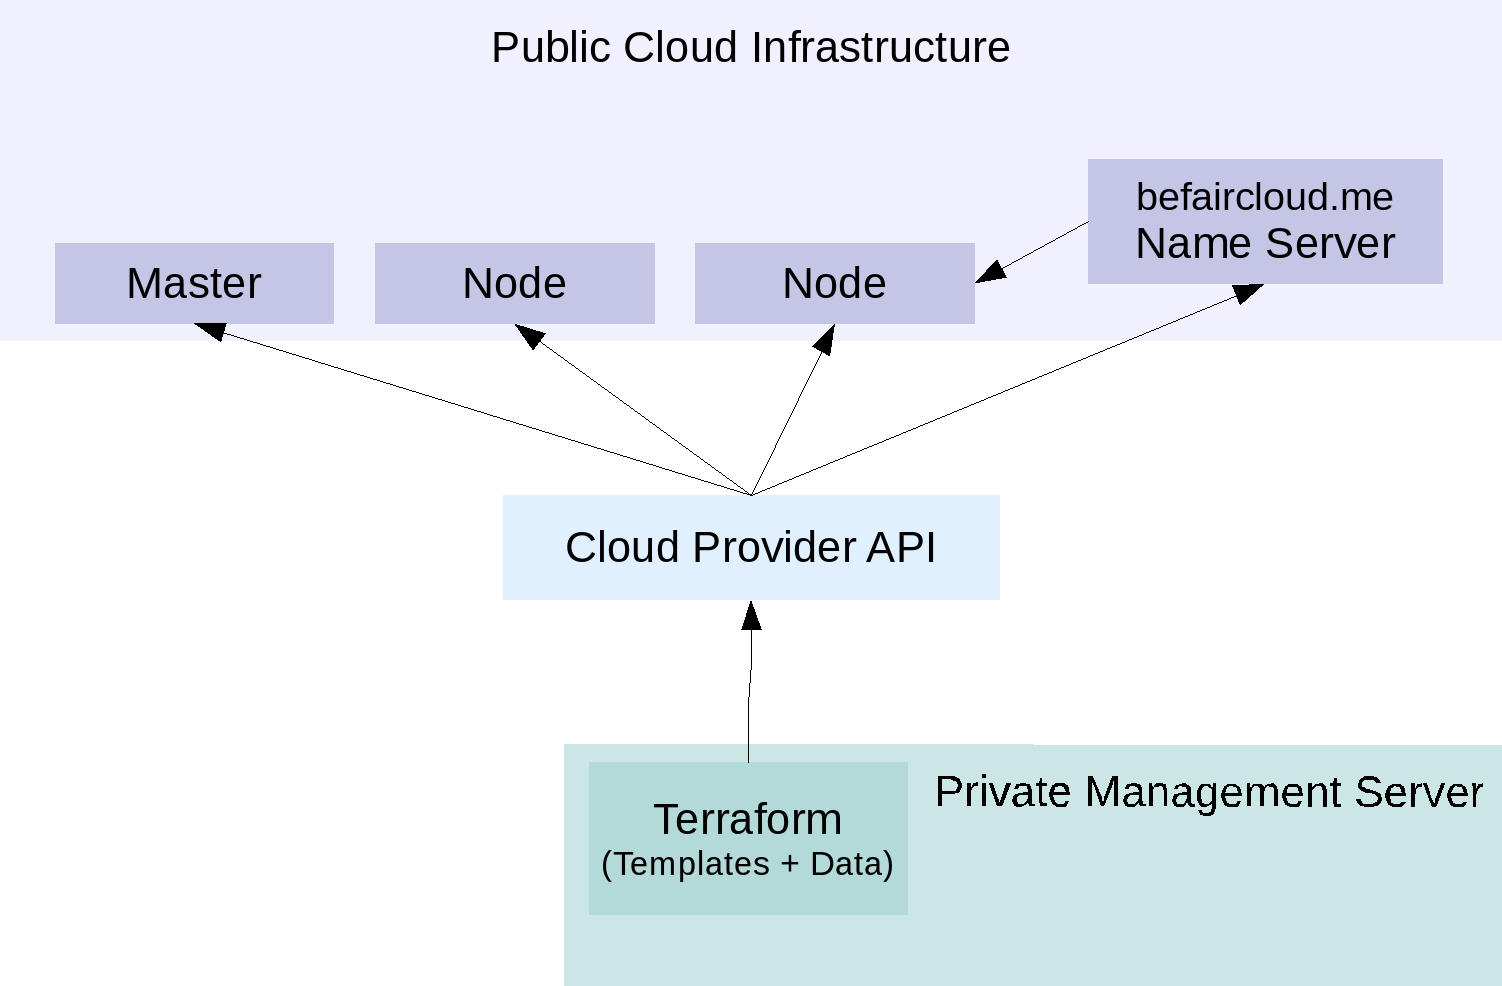
\includegraphics{media/ch4-terraform.png}
\caption{Infrastructure Provisioning with Terraform}
\end{figure}

Figure 4.3 shows the dependency graph of infrastructure resources, automatically generated by Terraform itself.

\begin{figure}[htbp]
\centering
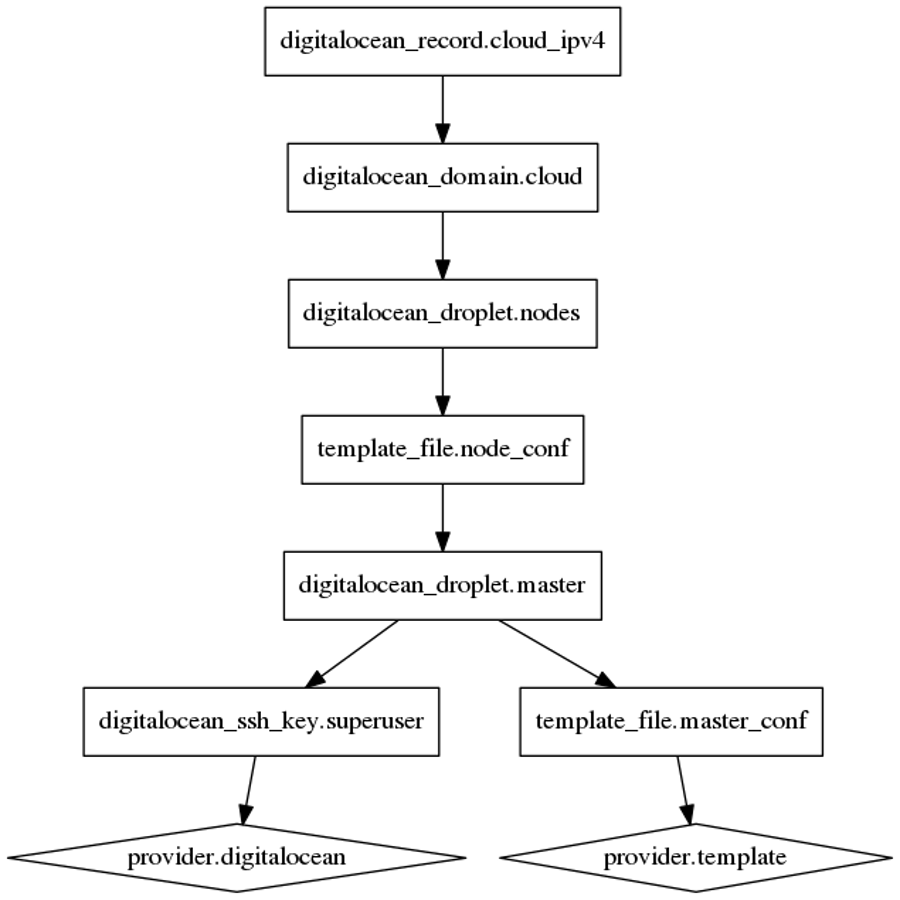
\includegraphics{media/ch4-graph.png}
\caption{Infrastructure Dependency Graph}
\end{figure}

All the Terraform configuration could be seen in the Appendix B.  Note that while Terraform supports custom language, the \textit{Hashicorp Configuration Language} (HCL) and JSON, the choice is to use a standardized, human-readable and clean YAML.

For launching all the infrastructure, it's so simple as running \texttt{make up}, that will do the following tasks:
\begin{enumerate}
\item cleaning previous temporary files;
\item compile YAML configurations into JSON;
\item creating a temporary SSH RSA 4096bit public/private key;
\item create an archive with necessary binaries and configuration files to upload on all hosts;
\item launching Terraform's \texttt{plan} in order to plans the operations to do;
\item launching Terraform's \texttt{apply} in order to apply the planned operations.
\end{enumerate}

At the end, there is some output with commands for complete the bootstrapping and log via SSH to master:

\begin{verbatim}
Outputs:

  step1 = scp -r core@46.101.133.104:./master .cache/; \
scp -r .cache/master core@46.101.138.191:./; \
scp -r .cache/master core@46.101.200.100:./

  step2 = log to master -- ssh core@46.101.133.104
log to node-0 -- ssh core@46.101.138.191
log to node-1 -- ssh core@46.101.200.100
dashboard -- https://46.101.133.104:8443
entrypoint -- http://befaircloud.me
\end{verbatim}

Now the whole cluster is up and running!

For enabling some basic services and monitoring stack, it's needed connecting via SSH to master, and running the \texttt{openshift/base} script, present on the home of the \texttt{core} user.

For deleting all resources (from VMs to DNS records), it's needed running \texttt{make destroy} that consists of:
\begin{enumerate}
\item \texttt{terraform plan -destroy} for planning deletion of all resources;
\item \texttt{terraform destroy} for deleting the planned destruction.
\end{enumerate}

\section{Provisioning of PaaS}\label{provisioning-of-paas}

Another core aspect to cover regards the PaaS bootstrapping, the process from vanilla CoreOS to a complete functioning clustered PaaS running Kubernetes and OpenShift.  There internals of cluster is so postponed to the next chapter.

The key technologies used is a combination of Terraform's template feature and Cloud Config\footnote{https://cloudinit.readthedocs.org/}, an emerging standard for operating system configuration at boot time via a declarative way.  Cloud Config consists of a simple YAML file that an OS (CoreOS, Ubuntu, etc.) could read, with information about hostname, ssh keys and user permissions, files and other settings.  CoreOS added additional features\footnote{https://coreos.com/os/docs/latest/cloud-config.html} for SystemD units and cluster upgrade.

Since master and node have a different configuration needs, there are been developed two templates.  Terraform use these templates and passing them when requesting the machines. The main dependency is provide the master private IPv4 address to nodes, so they can connect to the master.

The detailed steps for provisioning a master are:
\begin{enumerate}
\item Terraform resolves the Cloud Config template of master and resolves variables in the form \$\{VAR\_NAME\};
\item Terraform calls the API to pull up a new VM with vanilla CoreOS, passing the Cloud Config master, and uploading an archive (with necessary binaries and OpenShift configurations);
\item Digital Ocean parses this template replacing \$public\_ipv4 and \$private\_ipv4 variables;
\item Digital Ocean pulls up the master passing Cloud Config template to CoreOS;
\item CoreOS reads the full-rendered Cloud Config template, and apply the described configurations.
\end{enumerate}

Once the master has been correctly deployed, the nodes could be deployed:
\begin{enumerate}
\item Terraform resolves the Cloud Config template of node, passing the \textit{master IP}.  So this template could be used for every node for that specific master;
\item the same steps as for the master.
\end{enumerate}

The configuration described in Cloud Config is necessary for:
\begin{itemize}
\item enable SSH log-in to \texttt{core} user with provided key;
\item provide a SystemD unit for bootstrapping the host and write the OpenShift/Kubernetes configuration (different between master and node);
\item provide a SystemD unit for running the main OpenShift/Kubernetes binary (different between master and node).
\end{itemize}

Thanks to this capabilities, this entire process is (quite) totally automated, except for a single command, that is anyway automatically provided by Terraform at the end.

Figure 4.4 shows all the dependencies of PaaS bootstrapping, managed with a combination of Terraform, Cloud Config and SystemD units.

\begin{figure}[htbp]
\centering
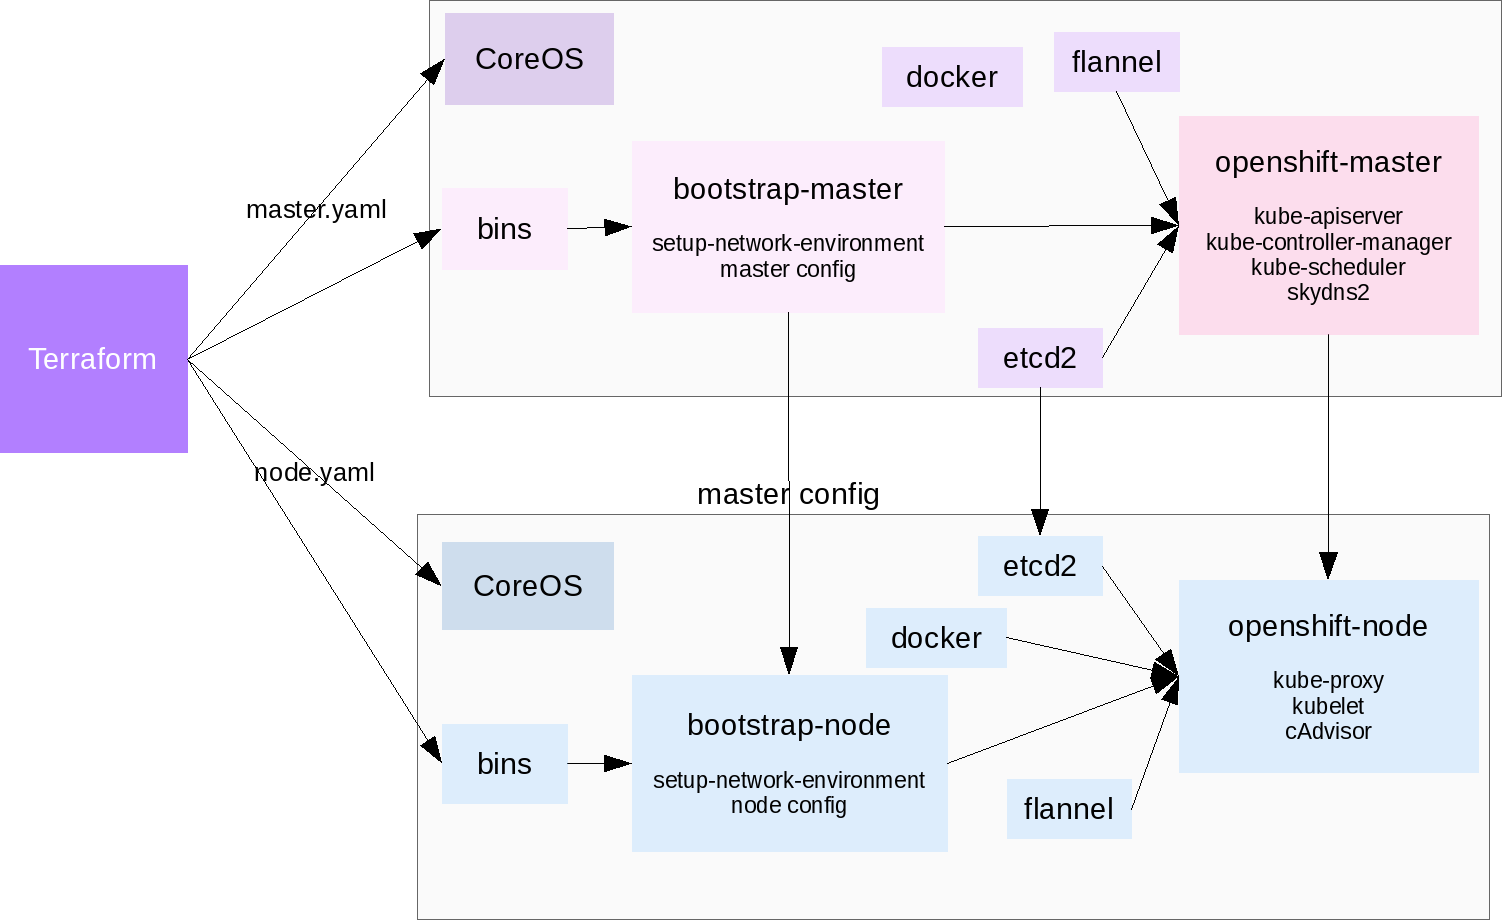
\includegraphics{media/ch4-bootstrap.png}
\caption{Provisioning of the PaaS}
\end{figure}